\section{System Overview}

\begin{outline}
  Present a high-level overview of your proposed control framework,
  likely including a block diagram (similar to Figure 1 in the
  proposal) and a description of each component.
\end{outline}

This work aims to take a footstep evaluation network, like ContactNet
from \cite{bratta_contactnet_2024}, and
extend it to provide dynamic gait generation capabilities. A footstep
evaluation network
ranks the cost of different footstep locations,

is able to generate acyclic gaits, which this work builds on top of
that to allow for moving multiple feet simultaneously. The proposed
framework is shown in \autoref{fig:diagram-control-system}.

\begin{todo}
  update the caption for \autoref{fig:diagram-control-system}
\end{todo}

\begin{figure}
  \centering
  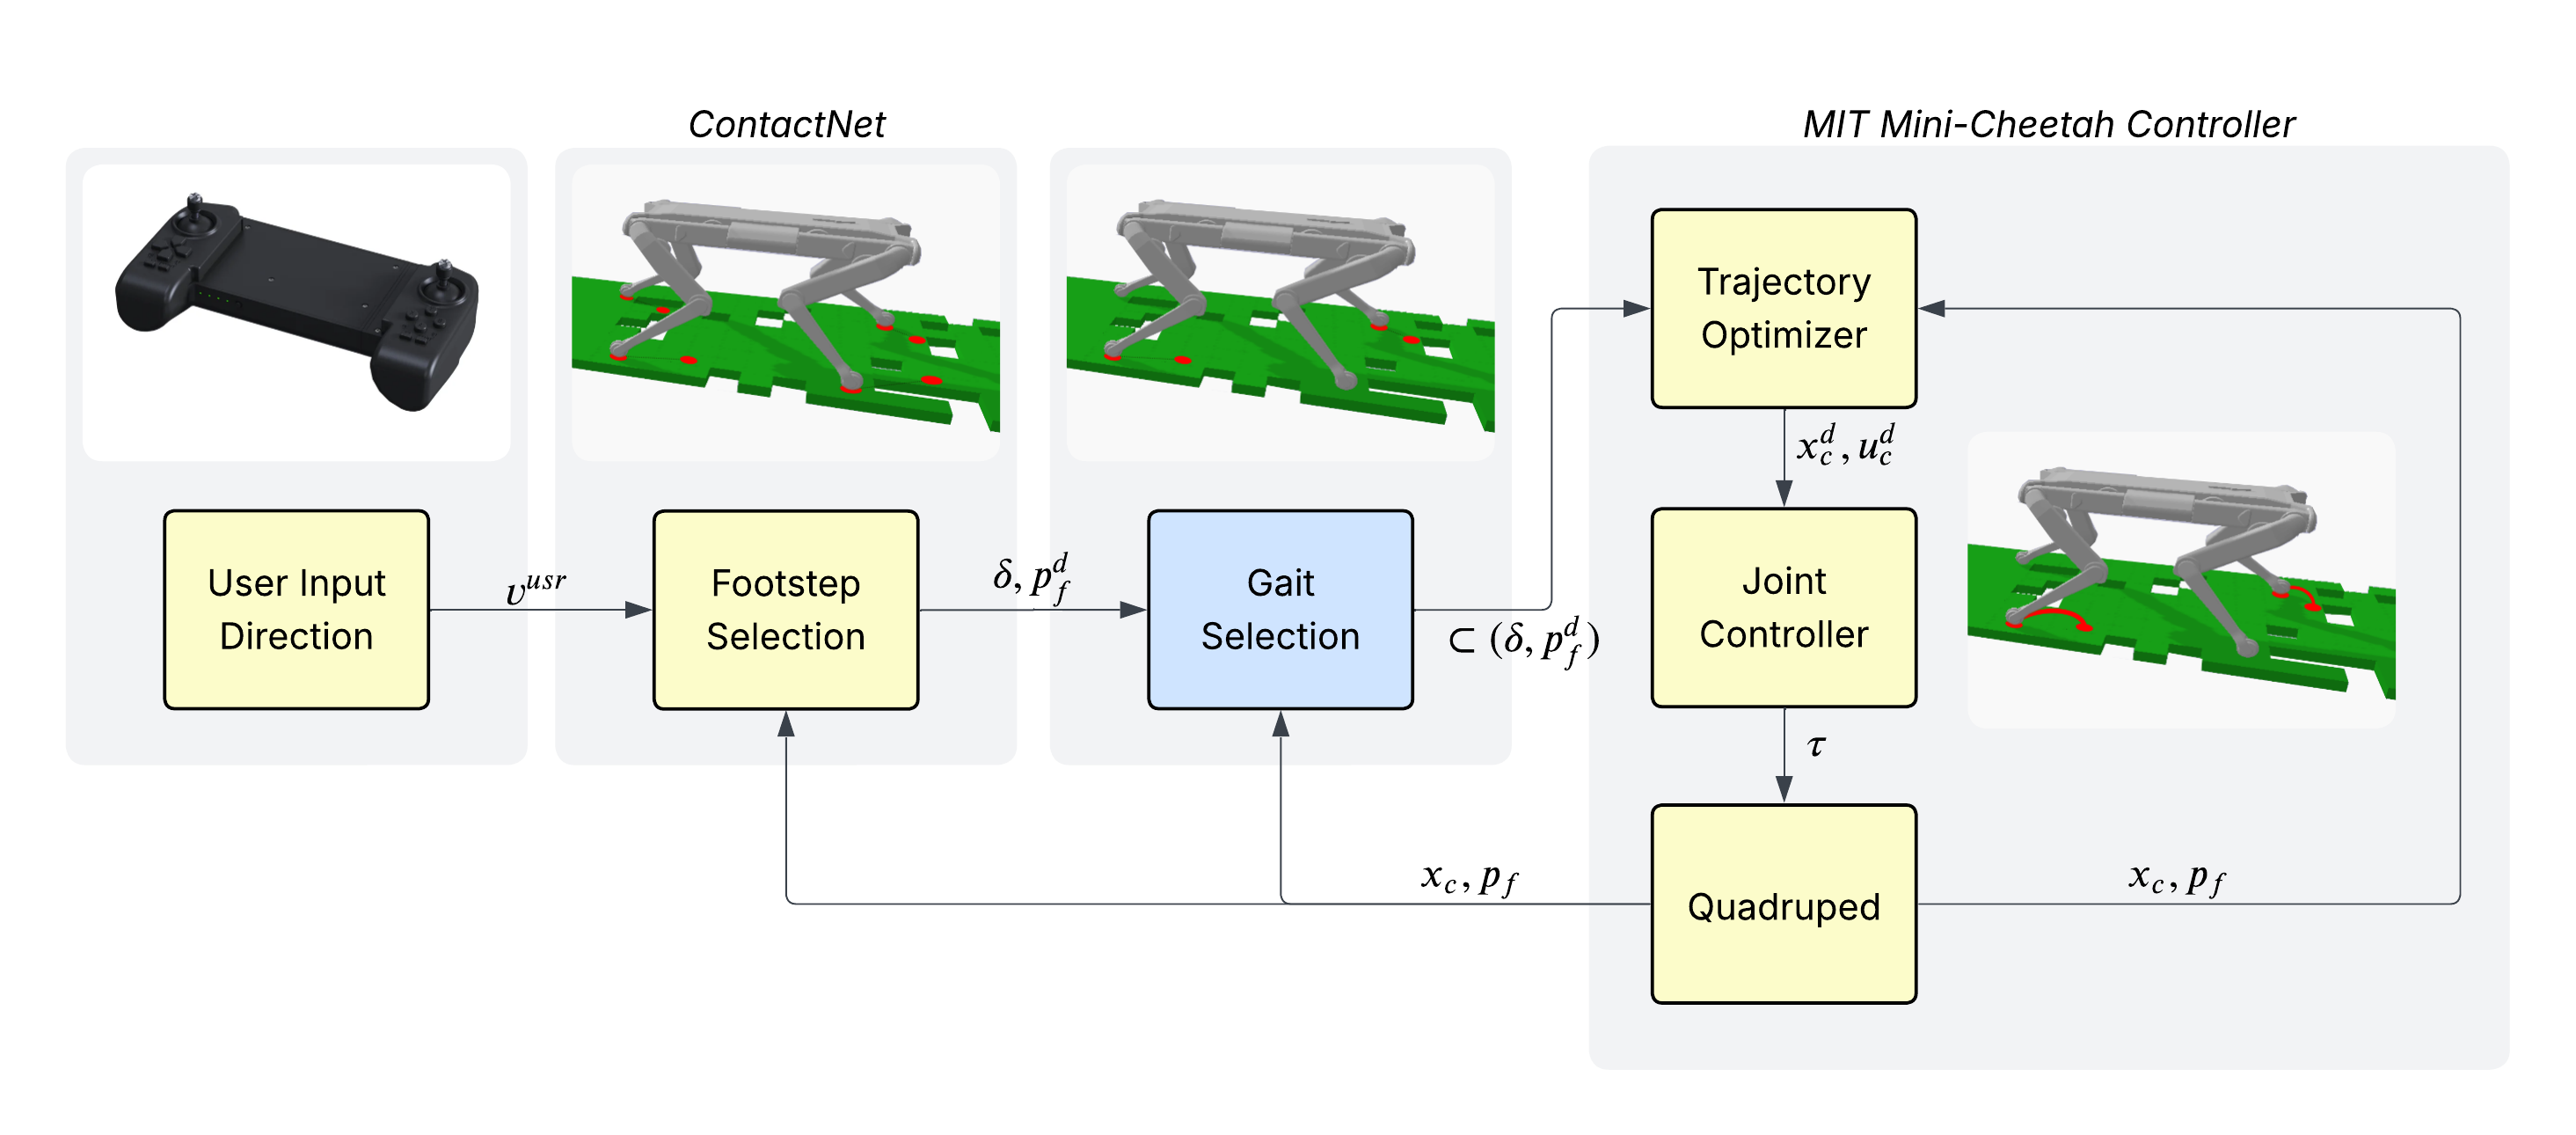
\includegraphics[width=1.0\linewidth]{images/diagrams/control-system.png}
  \caption{A block diagram of the proposed framework. The user
    defines an input direction $v^{usr}$ which the \textit{footstep
    selector} \cite{bratta_contactnet_2024} uses along with, the robot
    state $x_c$, and the current foot positions $p_f$ to generate the
    swing durations $\delta$ and touchdown points $p_f^d$ for all
    currently grounded feet. The \textit{gait selector} (novel) takes
    these desired foot movements and selects an appropriate subset
    $\subset(\delta,p_f^d)$ based on $x_c$, $p_f$, and the terrain
    data. $\subset(\delta,p_f^d)$ is then passed into the MIT
  Mini-Cheetah Controller as MPC constraints to perform lower level control.}
  \label{fig:diagram-control-system}
\end{figure}
